\documentclass[landscape,24pt, a0paper,colspace=10mm,blockverticalspace=12mm]{tikzposter}

% Bibliography
%\usepackage[backend=bibtex,firstinits=true,sorting=none, doi=false,isbn=false,url=false]{biblatex}
%\bibliography{Mendeley.bib}
%\renewbibmacro{in:}{}
%\DeclareFieldFormat*{title}{#1} 

% Bibliography v2
%\usepackage[style=nature,maxnames=1,uniquelist=false]{biblatex}
\usepackage[backend=bibtex,giveninits=true,sorting=none, doi=false,isbn=false,url=false,maxnames=1,uniquelist=false]{biblatex}
\renewbibmacro{in:}{}
\DeclareFieldFormat*{title}{#1} 

% For preventing hyphenation
\usepackage{hyphenat}
% e.g.    \nohyphens{longlineoftexthere}
    
% Some field suppression via options
\ExecuteBibliographyOptions{isbn=false,url=false,doi=false,eprint=false}

% One-paragraph bibliography environment
\defbibenvironment{bibliography}
  {\list
     {\printtext[labelnumberwidth]{%
        \printfield{labelprefix}%
        \printfield{labelnumber}}%
      \ifentrytype{article}{% Suppress remaining fields/names/lists here
        \clearfield{title}}{}}
     {\setlength{\leftmargin}{0pt}%
      \setlength{\topsep}{0pt}}%
      \renewcommand*{\makelabel}[1]{##1}}
  {\endlist}
  {\mkbibitem}

% \mkbibitem just prints item label and non-breakable space
\makeatletter
\newcommand{\mkbibitem}{\@itemlabel\addnbspace}
\makeatother

% Add breakable space between bibliography items
\renewcommand*{\finentrypunct}{\addperiod\space}

% et al. string upright (nature style applies \mkbibemph)
\renewbibmacro*{name:andothers}{%
  \ifboolexpr{
    test {\ifnumequal{\value{listcount}}{\value{liststop}}}
    and
    test \ifmorenames
  }
    {\ifnumgreater{\value{liststop}}{1}{\finalandcomma}{}%
     \andothersdelim
     \bibstring{andothers}}
    {}}

\addbibresource{Mendeley.bib}
 
 
%Remove 'references' title from bibliography
\usepackage{etoolbox}
\patchcmd{\thebibliography}{\section*{\refname}}{}{}{}

\usepackage{calculator}%For doing arithmetic?
\usepackage{verbatim}

\usepackage{amssymb, amsmath, mathrsfs, bm, mathtools}
\usepackage[makeroom]{cancel}

\newcommand{\Rm}{Rm}
\newcommand{\Da}{Da}
\newcommand{\Reynolds}{Re}
\newcommand{\Prandtl}{Pr}
\newcommand{\Ra}{Ra}

\newcommand{\St}{\mathscr{S}}
\newcommand{\ConcRatio}{\mathscr{C}}
\newcommand{\Le}{Le}


\newcommand*{\enthalpy}{\mathscr{H}}
\newcommand*{\RaT}{\ensuremath{Ra_T}}
\newcommand*{\RaTC}{\ensuremath{Ra_T^c}} %Critical rayleigh number
\newcommand*{\RaC}{\ensuremath{Ra_C}}
\newcommand*{\RaS}{\ensuremath{Ra_S}}
\newcommand*{\RmC}{\ensuremath{Rm_C}}
\newcommand*{\RmS}{\ensuremath{Rm_S}}
\newcommand*{\RmT}{\ensuremath{Rm_T}}
\newcommand*{\RmCrit}{\ensuremath{Rm_{crit}}}

\newcommand*{\Rmush}{\ensuremath{Rm}}
\newcommand*{\RaLiquid}{\ensuremath{Ra}}

\newcommand*{\RaCrit}{\ensuremath{Ra_c}}

\newcommand*{\Nu}{\ensuremath{Nu}}


\DeclareMathOperator\arctanh{arctanh}



% For displaying equations in tables
\usepackage{array}
%\def\tabularxcolumn#1{m{#1}} %ensure vertical centering
\newcolumntype{L}[1]{>{\raggedright\let\newline\\\arraybackslash\hspace{0pt}}m{#1}}
\newcolumntype{C}[1]{>{\centering\let\newline\\\arraybackslash\hspace{0pt}}m{#1}}
\newcolumntype{R}[1]{>{\raggedleft\let\newline\\\arraybackslash\hspace{0pt}}m{#1}}


\usepackage{authblk} %Formatting of author lists
\usepackage{enumitem} % For different itemize icons
\usepackage{graphicx,subcaption} % For subfigures
\usepackage{xcolor} %For colors in equations

%\definecolor{oxfordblue}{rgb}{0.0, 0.13, 0.28}
\definecolor{darkolivegreen}{rgb}{0.33, 0.42, 0.18}
\definecolor{darkmidnightblue}{rgb}{0.0, 0.2, 0.4}
\definecolor{darkpowderblue}{rgb}{0.0, 0.2, 0.6}
\definecolor{dodgerblue}{rgb}{0.12, 0.56, 1.0}
\definecolor{egyptianblue}{rgb}{0.06, 0.2, 0.65}
\definecolor{dukeblue}{rgb}{0.0, 0.0, 0.61}
\definecolor{falured}{rgb}{0.5, 0.09, 0.09}
\definecolor{royalfuchsia}{rgb}{0.79, 0.17, 0.57}

\definecolor{captiongray}{rgb}{0.15,0.15,0.15}
\definecolor{captionTitle}{rgb}{0, 0, 0}
\definecolor{dividingLines}{rgb}{0.7, 0.7, 0.7}
\definecolor{eqnLabelGray}{rgb}{0.3, 0.3, 0.3}


\newcommand{\figureTitle}[1]{\color{captionTitle}{\textbf{#1}} }
\newcommand{\figureCaption}[1]{\color{captiongray}{#1} }

\newcommand{\highlightText}[1]{\textcolor{dukeblue}{\textbf{#1}} }

\newcommand{\varColor}[1]{\textcolor{dukeblue}{#1}}
\newcommand{\eqnColor}[1]{\textcolor{royalfuchsia}{#1}}
\newcommand{\paramColor}[1]{\textcolor{falured}{#1}}
\newcommand{\varLabel}[1]{\textcolor{eqnLabelGray}{\text{#1}}}

\newcommand{\eqnLabel}[1]{\textcolor{eqnLabelGray}{#1}}

\usepackage{pgfplots}
\usepgfplotslibrary{fillbetween}
\pgfplotsset{compat=1.13}

\usepackage{tikz}
\usetikzlibrary{calc,positioning,decorations.markings, backgrounds}

\makeatletter

%24 pt for figure captions for AGU
\renewenvironment{tikzfigure}[1][]{
  \def \rememberparameter{#1}
  \vspace{10pt}
  \refstepcounter{figurecounter}
  \begin{center}
  }{
    \ifx\rememberparameter\@empty
    \else %nothing
    \\[24pt]
    {Fig.~\thefigurecounter: \rememberparameter}
    \fi
  \end{center}
}

% Title formatting
\def\TP@titlegraphictotitledistance{-5.0cm} % Without this, authors are below icons

\renewcommand\AB@affilsepx{, \protect\Affilfont}

\settitle{ \centering \vbox{

\centering
\vspace{-2.0cm}
\color{titlefgcolor} {\bfseries \Huge \sc \@title \par}
\vspace*{0.5cm} % Distance from bottom of title to top of graphics
% For title graphics. Uncomment next line to remove
\@titlegraphic \\ [\TP@titlegraphictotitledistance] 
{\LARGE \@author \par} \vspace*{0.8em} {\Large \@institute}
\vspace*{-5em}
}
}

\def\maketitle{\AB@maketitle} % prevent shifing content block to middle of page

\makeatother

%Define my block style
\defineblockstyle{MyBlock}{% define a custom style for a block
    titlewidthscale=1.0, bodywidthscale=1, titleleft,
    titleoffsetx=0pt, titleoffsety=0pt, bodyoffsetx=0pt, bodyoffsety=26mm,
    bodyverticalshift=16mm, roundedcorners=22, linewidth=5pt,
    titleinnersep=7mm, bodyinnersep=8mm
}{
    \draw[rounded corners=\blockroundedcorners, inner sep=\blockbodyinnersep,
          line width=\blocklinewidth, color=blocktitlefgcolor,
          top color=titlebgcolor, bottom color=titlebgcolor,
          fill=blockbodybgcolor
          ]
      (blockbody.south west) rectangle (blockbody.north east); %
    %\ifBlockHasTitle%
    %    \draw[rounded corners=\blockroundedcorners, inner sep=\blocktitleinnersep,
    %      top color=titlebgcolor!90, bottom color=titlebgcolor!20!white,
    %      line width=\blocklinewidth, color=black, %fill=blocktitlebgcolor
    %      ]
    %  (blocktitle.south west) rectangle (blocktitle.north east); %
    %\fi
}
\newcommand\myblock[3][MyBlock]{\useblockstyle{#1}\block{#2}{#3}\useblockstyle{Basic}}



% Theme details
\usetheme{Default} % See Section 5
\usebackgroundstyle{Empty}
\usetitlestyle[width=0.98\textwidth]{Default} 
\useblockstyle{MyBlock}

\definecolor{oxfordblue}{rgb}{0.0, 0.13, 0.28}

\definecolorstyle{sampleColorStyle} 
{
\definecolor{colorOne}{named}{blue}
\definecolor{colorTwo}{named}{yellow}
\definecolor{colorThree}{named}{orange} 
}{
% Background Colors
\colorlet{backgroundcolor}{white}
\colorlet{framecolor}{white}
% Title Colors
\colorlet{titlefgcolor}{oxfordblue}
\colorlet{titlebgcolor}{white} % white
% Block Colors
\colorlet{blocktitlebgcolor}{white} %oxfordblue
\colorlet{blocktitlefgcolor}{oxfordblue}
\colorlet{blockbodybgcolor}{oxfordblue} % white
\colorlet{blockbodyfgcolor}{black}
% Innerblock Colors
\colorlet{innerblocktitlebgcolor}{white}
\colorlet{innerblocktitlefgcolor}{black}
\colorlet{innerblockbodybgcolor}{colorThree!30!white}
\colorlet{innerblockbodyfgcolor}{black}
% Note colors
\colorlet{notefgcolor}{black}
\colorlet{notebgcolor}{colorTwo!50!white}
\colorlet{noteframecolor}{colorTwo}
}

\usecolorstyle[]{sampleColorStyle}

%\definecolor{MyYellow}{RGB}{175 141 38}

\usepackage{mdframed}
\newmdenv[topline=false,
leftline=false,
bottomline=false,
linewidth=1.5mm,
linecolor=oxfordblue,
skipabove=-20em,
innertopmargin=0em]{leftbot}


\usepackage{tcolorbox}
\tcbset{arc=20pt,
        leftright skip=-0.92em,
        after skip=-0.92em,
        boxrule=1.6mm}

%Title text and graphics
\title{\parbox{\linewidth}{\centering Modelling Convection, Phase Change and Salt Fluxes from Mushy Sea Ice}} %with Adaptive Mesh Refinement
\titlegraphic{ 
\includegraphics[height=4cm]{figures/AGU2018.eps} %TODO: update QR code

\includegraphics[height=4cm]{figures/Oxford.eps}

\includegraphics[height=4cm]{figures/Berkeley_Lab_Logo_Small.eps} 
 \hfill 
  
\includegraphics[height=4cm]{figures/nerc-logo.eps}  
     
\includegraphics[height=4cm]{figures/roysoclogo.jpg} 
}
%For now title graphic:
%\titlegraphic{}

% Authors
\author[1]{James Parkinson (james.parkinson@physics.ox.ac.uk)}
\author[1]{Andrew Wells}
\author[2]{Dan Martin}
\author[1]{Richard Katz}

\affil[1]{University of Oxford}
\affil[2]{Lawrence Berkeley National Laboratory}



\tikzposterlatexaffectionproofoff % get rid of watermark in bottom right corner


 \tikzset{->-/.style={decoration={
  markings,
  mark=at position .5 with {\arrow[scale=2]{latex}}},postaction={decorate}}}





\begin{document}


\maketitle

\begin{columns} 

\column{0.21}

\block{Introduction}{
\begin{itemize}[leftmargin=0.4cm]
    %\item 22 million square kilometres of sea ice form every year \cite{fetterer-02}
    \item Sea ice is a mushy layer of ice crystals and brine.
    \item Dense brine drains during ice formation (Fig. 1), affecting ocean circulation. \\
    \textbf{Our goal: constrain brine fluxes} using numerical simulations.
    %\item We use a \textbf{low concentration ratio}, \\ $\ConcRatio \approx S_\text{ocean}/(S_\text{eutectic} - S_\text{ocean}) \ll 1$, \\ as is appropriate for sea ice.
\end{itemize}

\vspace{-0.0cm}

\begin{tikzfigure}
%[Mushy layer grown in a lab, $\sim$10cm deep. \\ (Schulze \& Worster, 1998) %\cite{Schulze1998}]
\label{fig:lab-mushy-layer}
%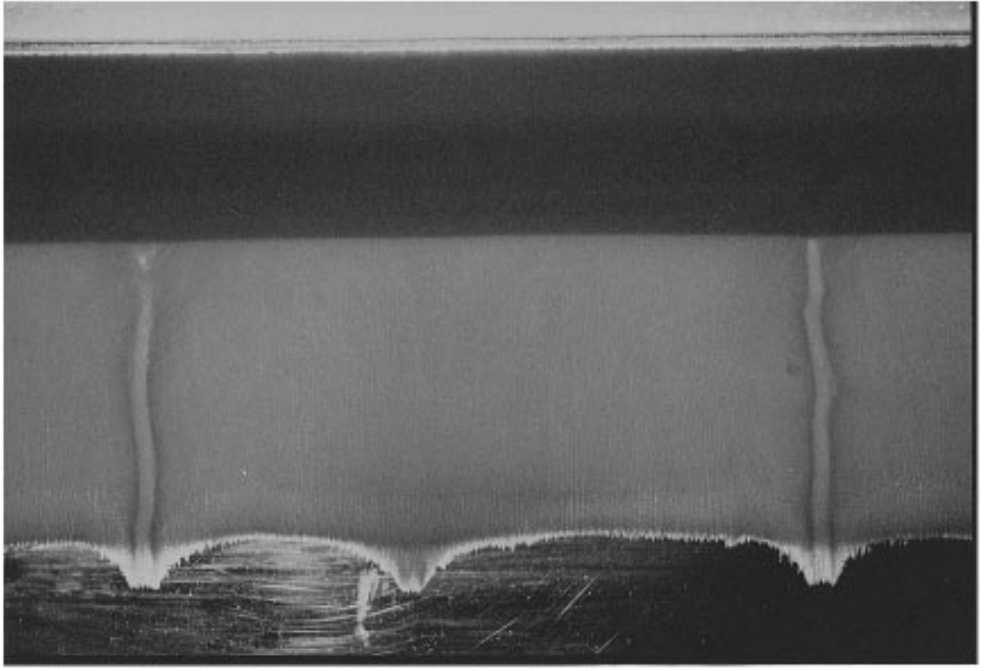
\includegraphics[width=\linewidth]{../Images/SchulzeWorsterMushyLayer.png}  \vspace{-2em}
\begin{tikzpicture}
\node[anchor=north west] (fig1) at (0,0) {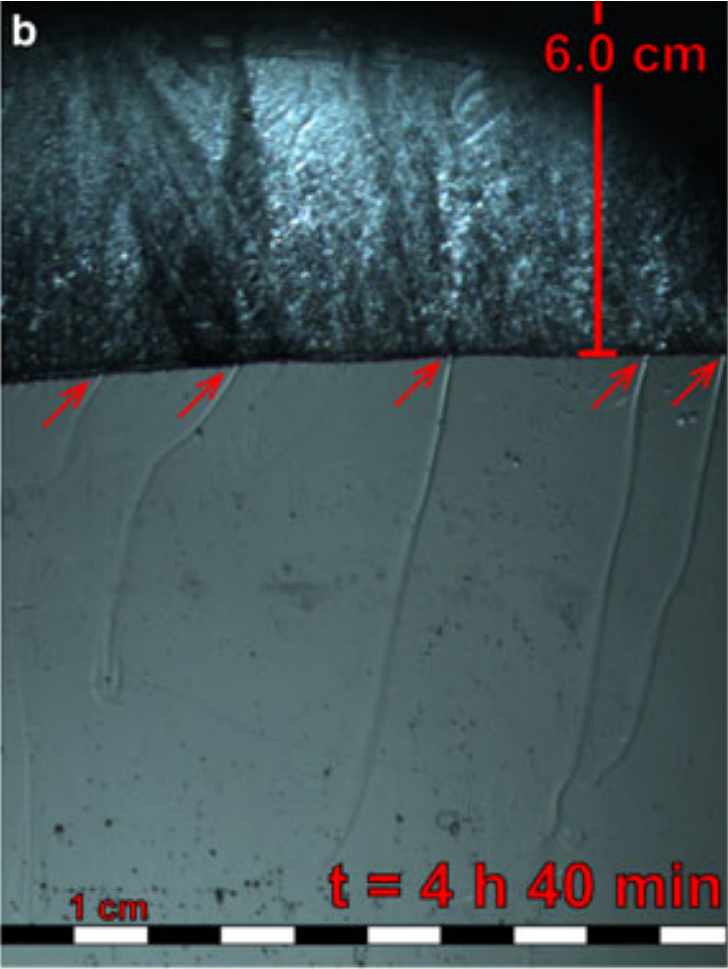
\includegraphics[width=10.5em, trim={0.0cm, 8.0cm, 0.0cm, 0.0cm}, clip]{figures/MiddletonEtAlBrineChannels.png} }; %0.47 \linewidth

%\node[anchor=north west] (fig2) at (fig1.north east) {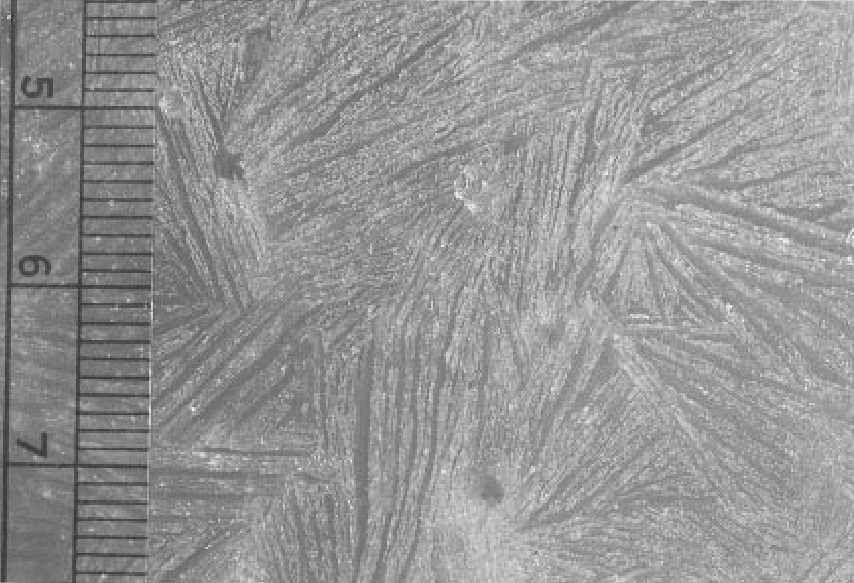
\includegraphics[width=0.55\linewidth, trim={0.0cm, 0cm, 0cm, 0cm}, clip]{figures/Wettlaufer1997BrineChannel.png} };
%\draw[red, line width = 2mm, ->] ([xshift=0cm, yshift=-2.0cm]fig2.north) -- ([xshift=-3.2cm, yshift=-3.2cm]fig2.north);
%\draw[red, line width = 2mm, ->] ([xshift=4.0cm, yshift=-7.0cm]fig2.north) -- ([xshift=1.5cm, yshift=2.1cm]fig2.south);

\node[anchor=north west] (fig2) at (fig1.north east) {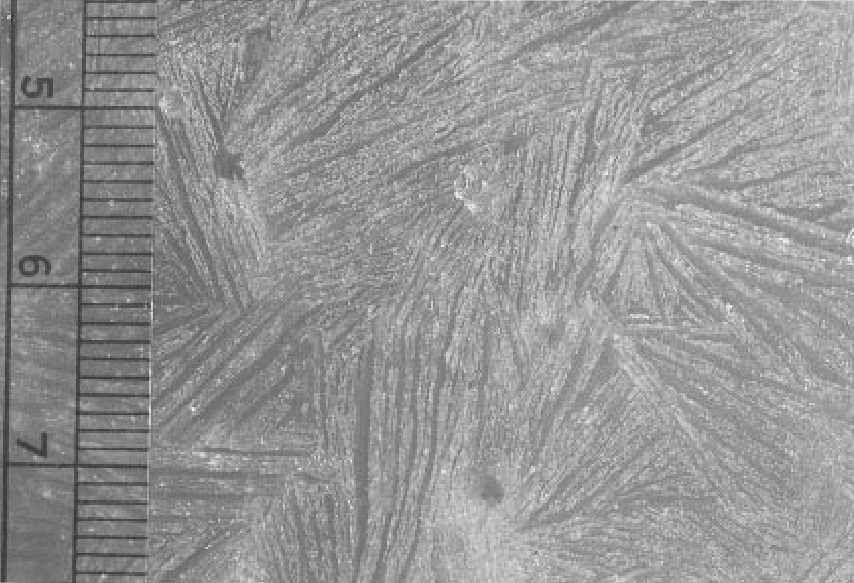
\includegraphics[angle=90,origin=c, width=10em, trim={0.0cm, 0.0cm, 8.0cm, 0cm}, clip]{figures/Wettlaufer1997BrineChannel.png} }; %0.455\linewidth
% Bottom left arrow
\draw[red, line width = 2mm, ->] ([xshift=-1.0cm, yshift=-4.0cm]fig2.north) -- ([xshift=3.1cm, yshift=-1.1cm]fig2.west);
% Top right arrow
\draw[red, line width = 2mm, ->] ([xshift=-3.0cm, yshift=0.0cm]fig2.east) -- ([xshift=-1.95cm, yshift=2.6cm]fig2.east);

\node[anchor=north west,fill=white!100,outer sep=0cm] at (fig1.north west) {(a)};
\node[anchor=north west,fill=white!100,outer sep=0cm] at (fig2.north west) {(b)};

\end{tikzpicture}
\end{tikzfigure}
\figureTitle{Fig. 1:} \figureCaption{Solidification of salt water viewed from (a) side; Middleton et. al. (2016) and (b) below; Wettlaufer et. al. (1997). Arrows indicate where salty plumes leave the ice. } 

}


\block{What is a mushy layer?}
{
\vspace{-0cm}
\begin{tikzfigure}
\label{fig:phaseDiagram}
\begin{tikzpicture}

\node[anchor=north west] (fig2) at (0,0) {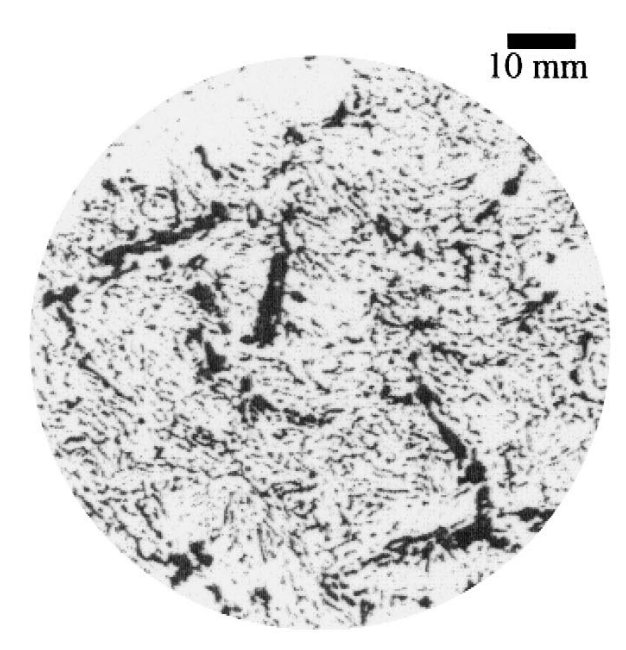
\includegraphics[width=0.4\linewidth, trim={0.0cm, 0.0cm, 0.0cm, 0.0cm}, clip]{figures/Eicken2000Edited.jpg} };

\node[anchor=north west] (phaseDiagram) at ([xshift=1.0cm]fig2.north east) {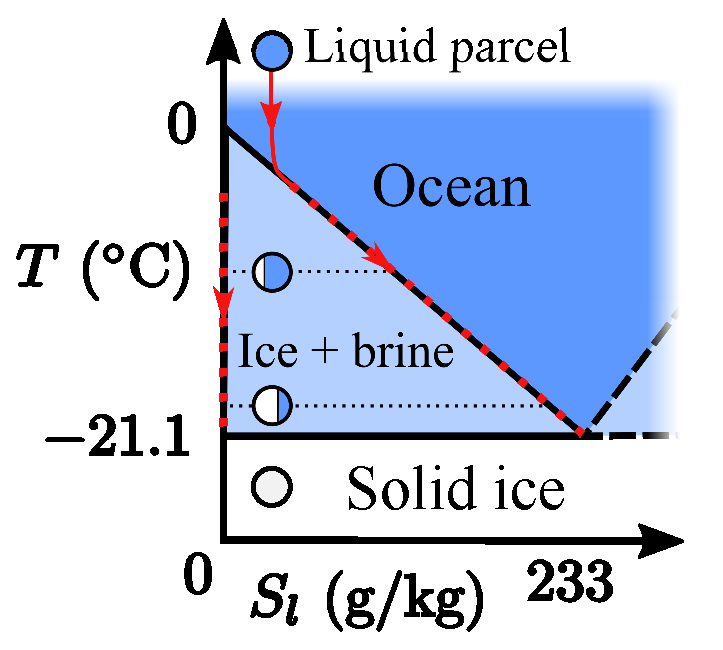
\includegraphics[width=0.47\linewidth, trim={0.0cm, 0.0cm, 0.0cm, 0.0cm}, clip]{figures/phaseDiagramVFinal.eps} };

\node[anchor=north west] (fig2label) at (fig2.north west) {(a)};

\node[anchor=north west] (fig1label) at ([yshift=0.0cm]phaseDiagram.north west) {(b)};

\end{tikzpicture}
\end{tikzfigure}
\figureTitle{Fig. 2:} \figureCaption{(a) Sea ice is a porous mixture of solid ice crystals (white) and liquid brine (dark) \cite{Eicken2000}. (b) Trajectory ($\textcolor{red}{\rightarrow}$) of a solidifying salt water parcel through the phase diagram. As the temperature $T_l$ decreases, more ice forms and the residual brine salinity $S_l$ increases making the fluid denser, which can drive convection. Below the eutectic ($T_e, S_e$) = (-21.1$^\circ$, 233) the system is entirely solid.} %making the fluid denser which can lead to convection
%the resulting dense fluid can drive convection
%Eicken et. al. (2000).
}
\block{Numerical Method}
{
\vspace{0.5em}
Solve (1)-(4) using Chombo finite volume toolkit:
\begin{itemize}
    \item Momentum and mass: projection method \cite{Martin2008}.
    \item Energy and solute:
    
%     \hspace{-\baselineskip}
%     \begin{minipage}[t]{8cm}
%     \textit{Advective terms:}  \\
%     explicit, 2\textsuperscript{nd} order unsplit Godunov.
%     \end{minipage} \hfill \vrule{} \hfill
%     \begin{minipage}[t]{12cm}
%     \textit{Nonlinear diffusive terms: } \\
%     semi implicit, geometric multigrid.
%     \end{minipage}

%    \item Timestepping: Backward Euler.

    %\nohyphens{
    {
    \raggedright % left align - prevent splitting words over multiple lines as we have space
   \begin{itemize}    
   \item Advective terms: explicit, 2\textsuperscript{nd} order unsplit Godunov method. %\cite{Colella1990}, 
   \item Nonlinear diffusive terms: semi implicit, geometric multigrid. %\cite{Martin1996}
   \item Timestepping: Backward Euler. %\cite{Twizell1996} 
   \end{itemize}
   }
  % }
\end{itemize}
\vspace{-1ex}
}




\block[bodyoffsety=0mm, bodyverticalshift=0mm]{}{ %Need to specify some options to get rid of the title space
This work was funded by NERC and a travel grant from the Royal Society.
{
\fontsize{16}{15}\selectfont 
\renewcommand\refname{\vskip -2.5cm}
%\bibliography{bibliography}
\renewcommand*{\bibfont}{\scriptsize}
\printbibliography
}
\vspace{-0.75cm}
}

%\column{0.55}
%\column{0.42}
\column{0.79}


%\block{Scaling laws for confined convection}{
\block{}{

 
\begin{tcolorbox}[width=0.49\linewidth, nobeforeafter, box align=top, bottomrule=0pt,toprule=0pt, leftrule=0.0pt, sharp corners=east, colframe=oxfordblue, colback=white, left skip=0.75pt, before skip=-2.4em, top=0.4em, left=0.0em, standard jigsaw, opacityback=0, extrude left by=0.9em, arc=6mm]

\begin{tcolorbox}[boxsep=5mm, width=1.016\linewidth,  sharp corners=uphill,
        colback=red!5,
        colframe=red!60!black, before skip=-2.5em, after skip=0.5em, left skip=-1.055em, boxrule=1.5mm, extrude top by=0.7em, arc=6mm]
%\LARGE \textbf{Conclusions:}
\vspace{-1.0em}
\begin{minipage}[c]{9cm}

\vspace{-1.5em}
\LARGE \textbf{Summary:}

\end{minipage}\hfill
\begin{minipage}[c]{\linewidth - 9cm}
\large 
\begin{itemize}
\item \textbf{During transient growth, channel spacing increases over time.} 
\item \textbf{Scaling predictions for steady state growth are consistent with experimental observations}
\end{itemize}
\end{minipage}
\vspace{-0.5em}
\end{tcolorbox}



{\LARGE \textcolor{oxfordblue}{\textbf{Simulated transient growth}}}

Water of initial salinity $S_0=35\,\mathrm{g\,kg}^{-1}$ and temperature $-2^\circ$C is frozen from above in a Hele-Shaw cell (plate separation $d=1$mm). We assume $K_0=10^{-9}\,\mathrm{m}^2$, and vary the atmospheric temperature $T_a$.
%\vspace{-4.5em}
\vspace{0.2em}
\textcolor{dividingLines}{\hrule}
%\vspace{-0.2em}
%\textcolor{dividingLines}{\rule{\linewidth}{0.2pt}}
%\vspace{-1em}
%\vspace{0.5em}
\hspace{-0.6cm}\begin{minipage}[t]{27.8cm}
\begin{tikzfigure}
\begin{tikzpicture} 
\node[anchor=north west, inner sep=0pt, outer sep=0pt] (timeseries) at (0,0) {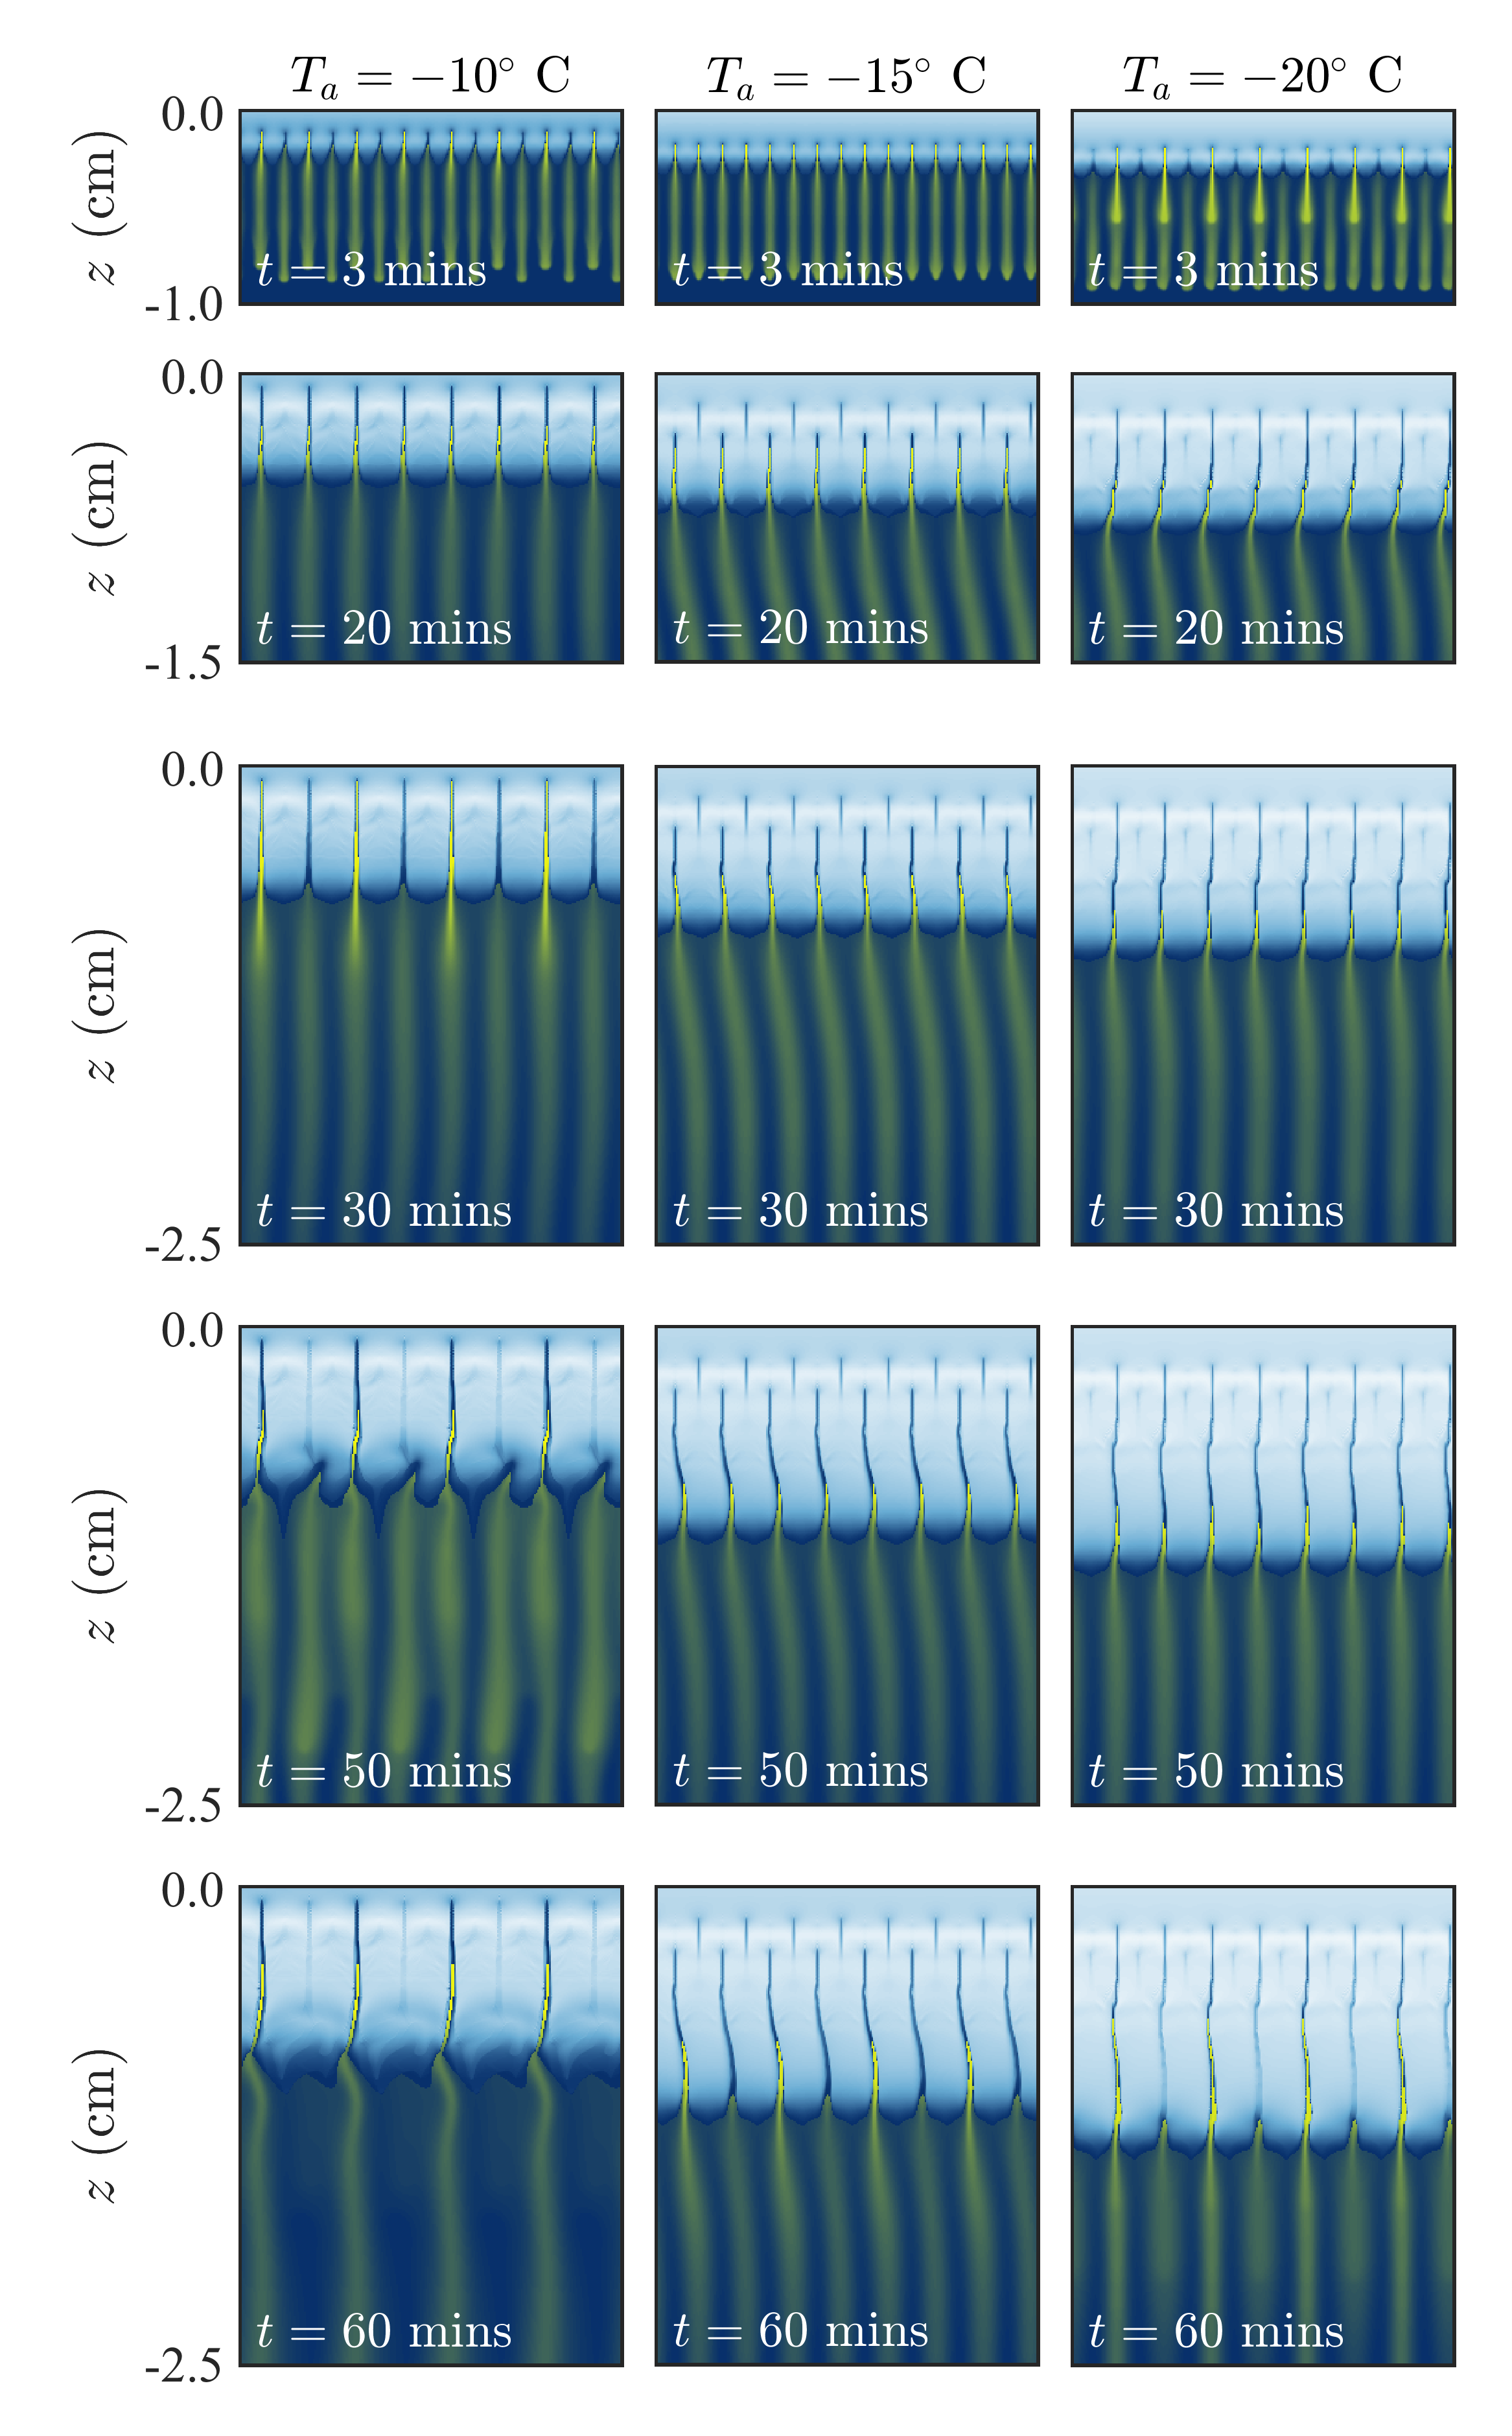
\includegraphics[width=28cm, trim={0.5cm, 0.5cm, 0.5cm, 0.5cm}, clip]{figures/timeSeries-t.png} };
\node[anchor=north west, inner sep=0pt, outer sep=0pt] (timeseries) at ([xshift=0cm,yshift=-0.3cm]timeseries.south west) 
{\figureTitle{Fig. 4:}\figureCaption{Ice grown from a fixed boundary.  https://goo.gl/4n9STV}};
\end{tikzpicture}
\end{tikzfigure} 
 



\end{minipage} \hfill \textcolor{dividingLines}{\vline} \hfill
\begin{minipage}[t]{15.0cm}

\begin{tikzfigure}
\begin{tikzpicture}
\node[anchor=north west, inner sep=0pt, outer sep=0pt] (BCs) at (0,0) {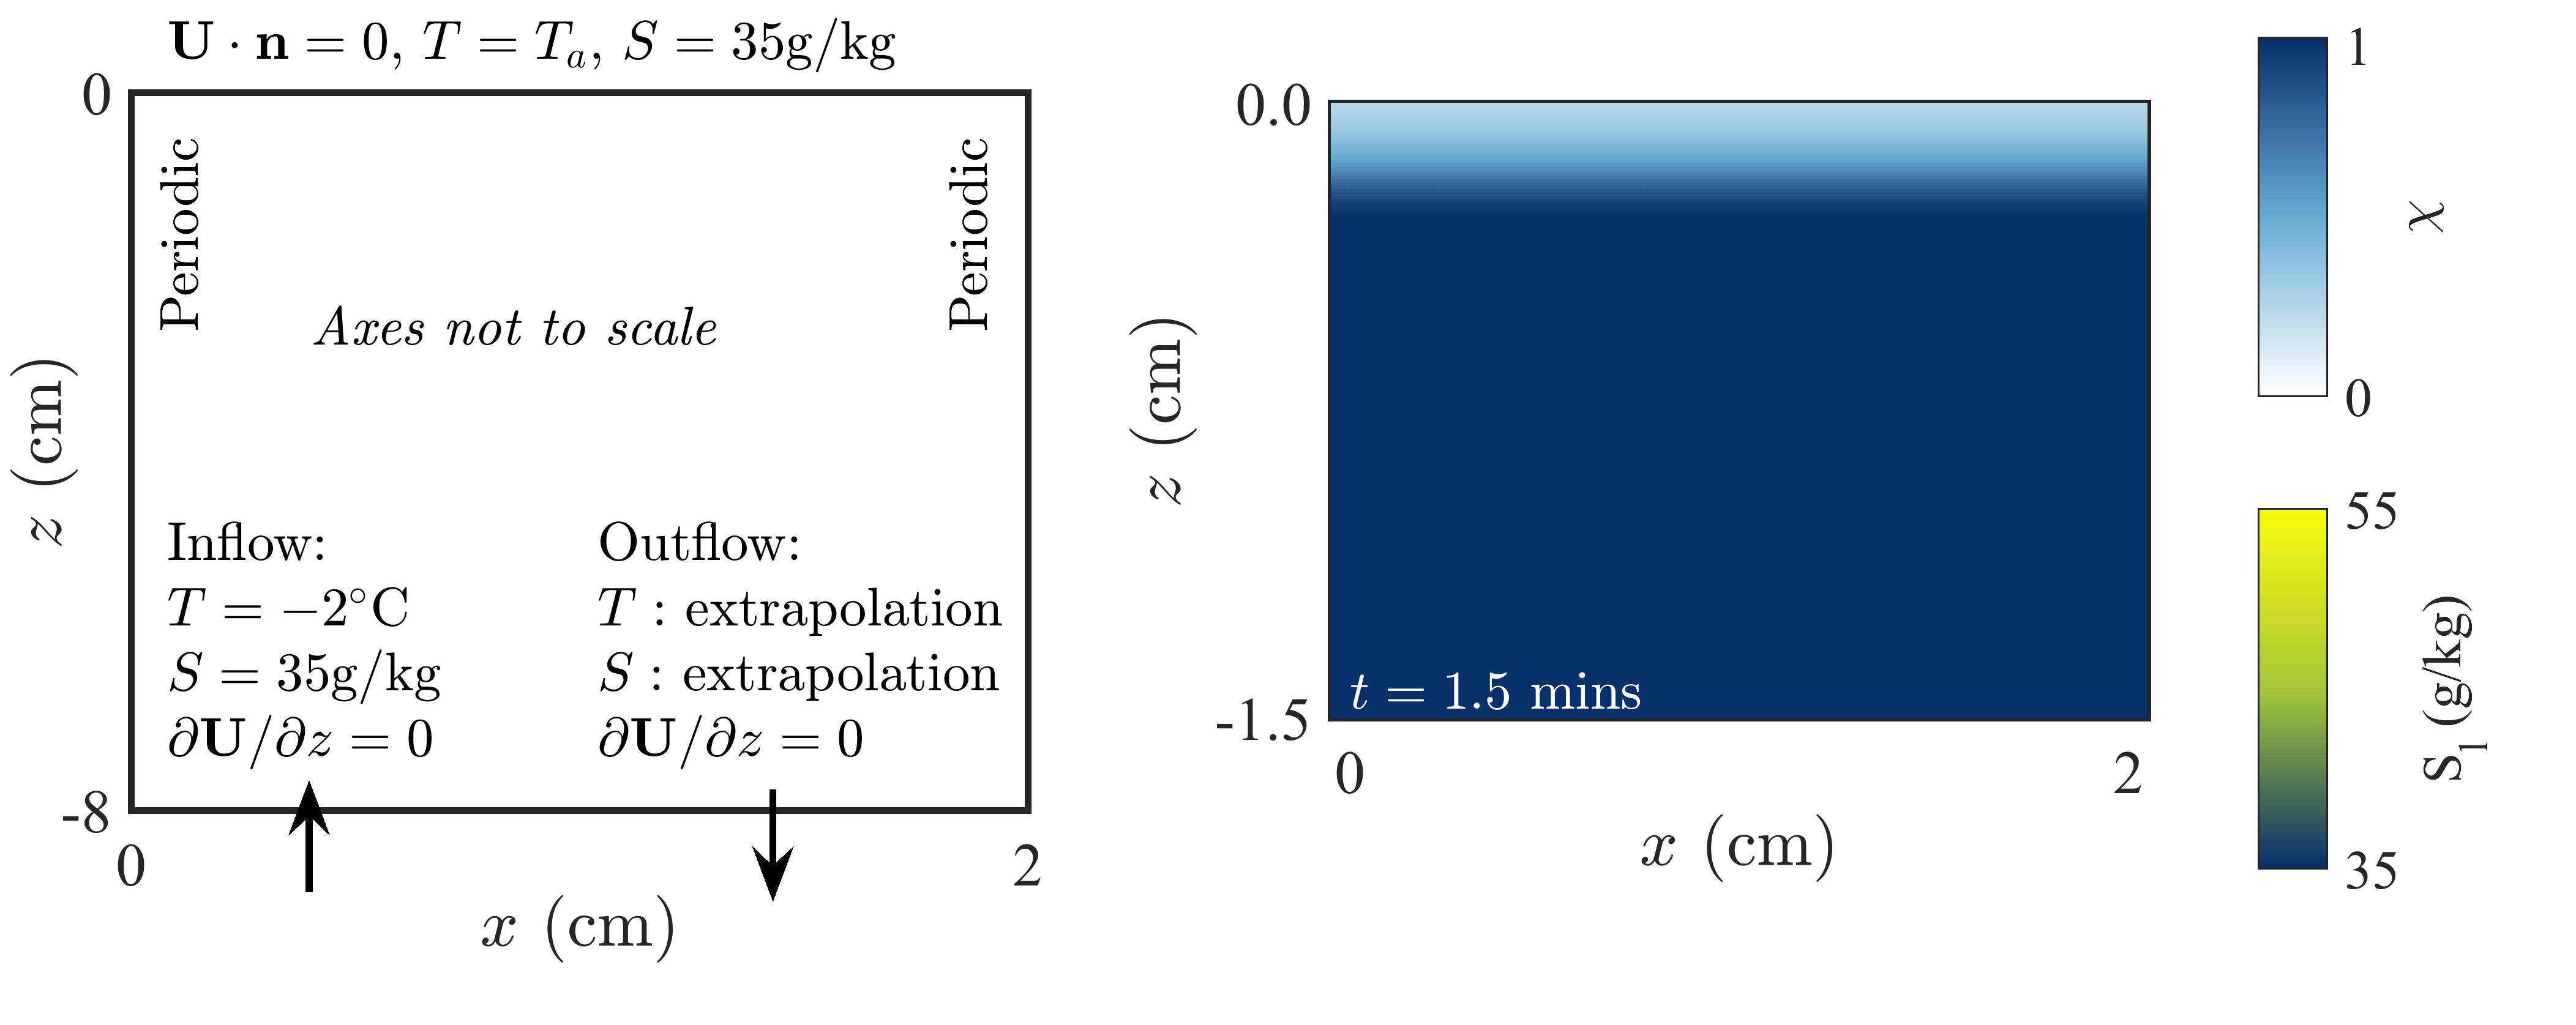
\includegraphics[height=12cm, trim={0.0cm, 0, 15.5cm, 0}, clip]{figures/EGUBCs.png} };

\node[anchor=north west, inner sep=0pt, outer sep=0pt] (BCs) at (BCs.north east) {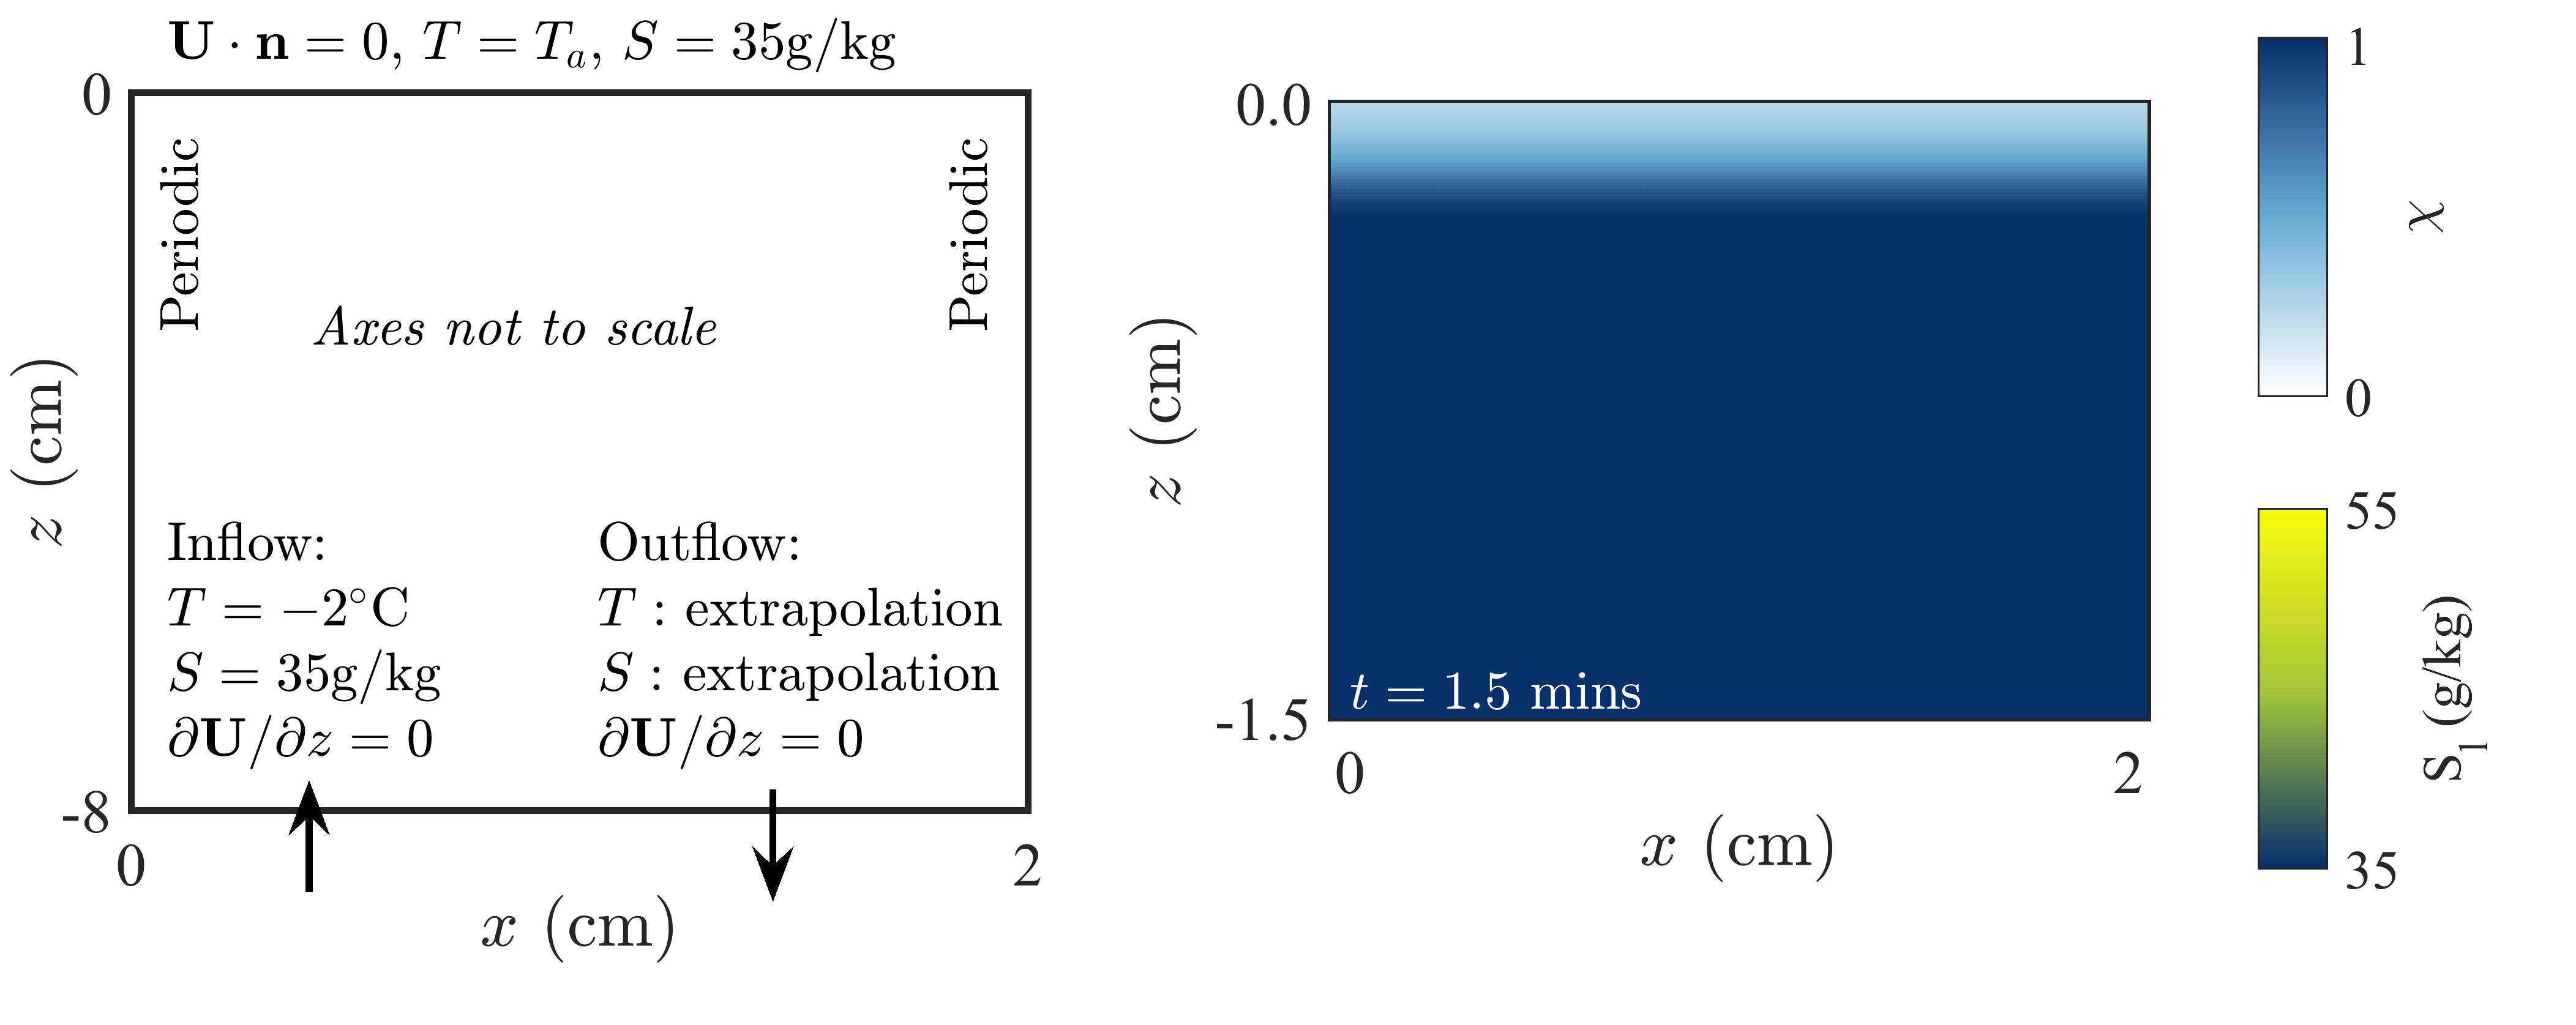
\includegraphics[height=12cm, trim={23.4cm, 0, 1.0cm, 0}, clip]{figures/EGUBCs.png} };

%\node[anchor=south west, inner sep=0pt, outer sep=0pt] (aLabel) at ([xshift=-0.5cm, yshift=-0.8cm]BCs.north west) {(a)};

%\node[anchor=south west, inner sep=0pt, outer sep=0pt] (bLabel) at ([xshift=0.5cm, yshift=-0.8cm]BCs.north) {(b)};
\end{tikzpicture}
\end{tikzfigure}
\vspace{-0.3\baselineskip}
\figureTitle{Fig. 3 ($\uparrow$).}\figureCaption{Domain and colorbars for transient simulations ($\leftarrow$).}
%(b) Solution for $T_a=-15^\circ$C, before the onset of convection.
\vspace{0.3em}
\textcolor{dividingLines}{\hrule}
\vspace{-0.3em}
\begin{tikzfigure}
\begin{tikzpicture}
\node[anchor=north west, inner sep=0pt, outer sep=0pt] (BCs) at (0,0) {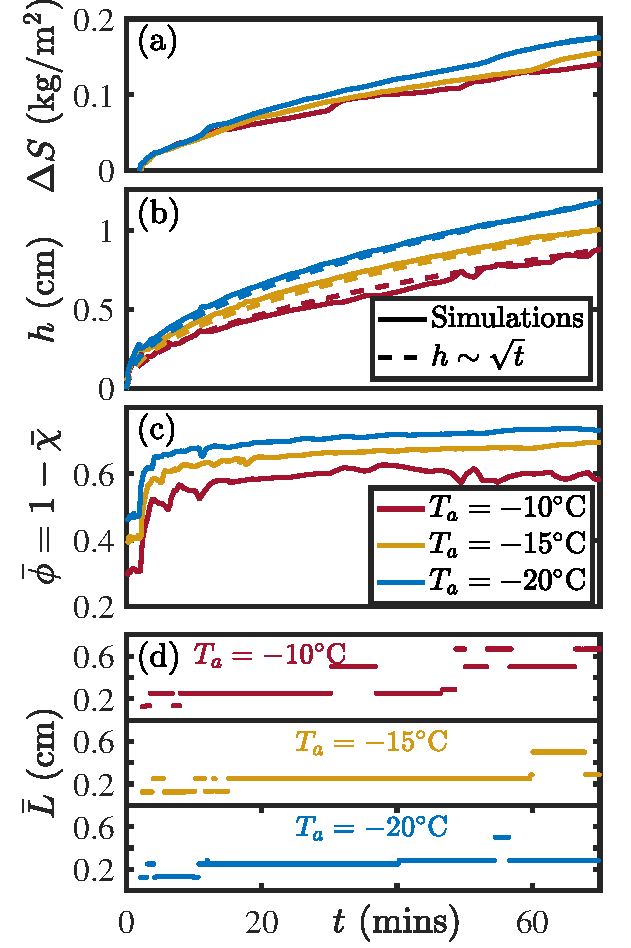
\includegraphics[width=15.2cm, trim={0.0cm, 0, 0.0cm, 0}, clip]{figures/transientDiagnosticsExtended.pdf} }; 


\end{tikzpicture}
\end{tikzfigure}
\figureTitle{Fig. 5 ($\uparrow$).}\figureCaption{(a) Total salt rejected from ice. (b) Ice depth increases roughly $\propto \sqrt{t}$. (c) Average solid fraction $\bar{\phi}$ increases following the onset of convection. (d) Average channel spacing $\bar{L}$ increases over time.  }

\end{minipage}

\iffalse
\begin{tcolorbox}[boxsep=5mm, width=1.016\linewidth,  sharp corners=downhill,
        colback=red!5,
        colframe=red!60!black, before skip=0.5em, after skip=-2em, left skip=-1.055em, boxrule=1.5mm, extrude bottom by=1.25em, arc=6mm]
%\LARGE \textbf{Conclusions:} 
\begin{minipage}[c]{9cm}
\vspace{-0.5em}
\LARGE \textbf{Summary:}

\end{minipage}\hfill
\begin{minipage}[c]{\linewidth - 9cm}
\large 
\begin{itemize}
\item \textbf{During transient growth, channel spacing increases over time.} 
\item \textbf{Scaling predictions for steady state growth are consistent with experimental observations}
\end{itemize}
\end{minipage}
\vspace{-1.8em}
\end{tcolorbox}
\fi

\end{tcolorbox} \hfill
\begin{tcolorbox}[width=0.49\linewidth, nobeforeafter, box align=top, boxrule=0mm, colback=white, colframe=white, right skip=0.75pt, top=0.4em, left=-1.0em, standard jigsaw, opacityback=0]
{\LARGE \textcolor{oxfordblue}{\textbf{Steady state solutions}} }

\begin{minipage}[t]{0.54\linewidth}
%\vspace{10pt}
For ice grown at a constant rate $V$ from water of initial salinity $S_0$ we investigate the sensitivity to the Rayleigh number $Rm$ and concentration ratio $\mathcal{C}$,
\begin{align}
   \textcolor{dukeblue}{ \mathcal{C} = \frac{S_0}{S_e - S_0}.} \nonumber
\end{align}


In fig. 6 (right $\rightarrow$), we plot the porosity $\chi$, streamlines (white) and salinity contours (red) for steady state solutions, where the domain width is chosen to maximise the solute flux. \highlightText{Decreasing $\mathcal{C}$ reduces the porosity, confining convection to a narrow porous layer at the mush-liquid interface.} \\

Below, we construct a scaling argument for $\mathcal{C} \ll 1$, then compare to numerical simulations (fig. 7) and experimental results (fig. 8).

\end{minipage} \hfill
\begin{minipage}[t]{0.49\linewidth}
\vspace{-3em} 
\begin{tikzfigure}
\begin{tikzpicture}
%\node[anchor=north west, inner sep=0pt, outer sep=0pt] (timeseries) at (0,0) {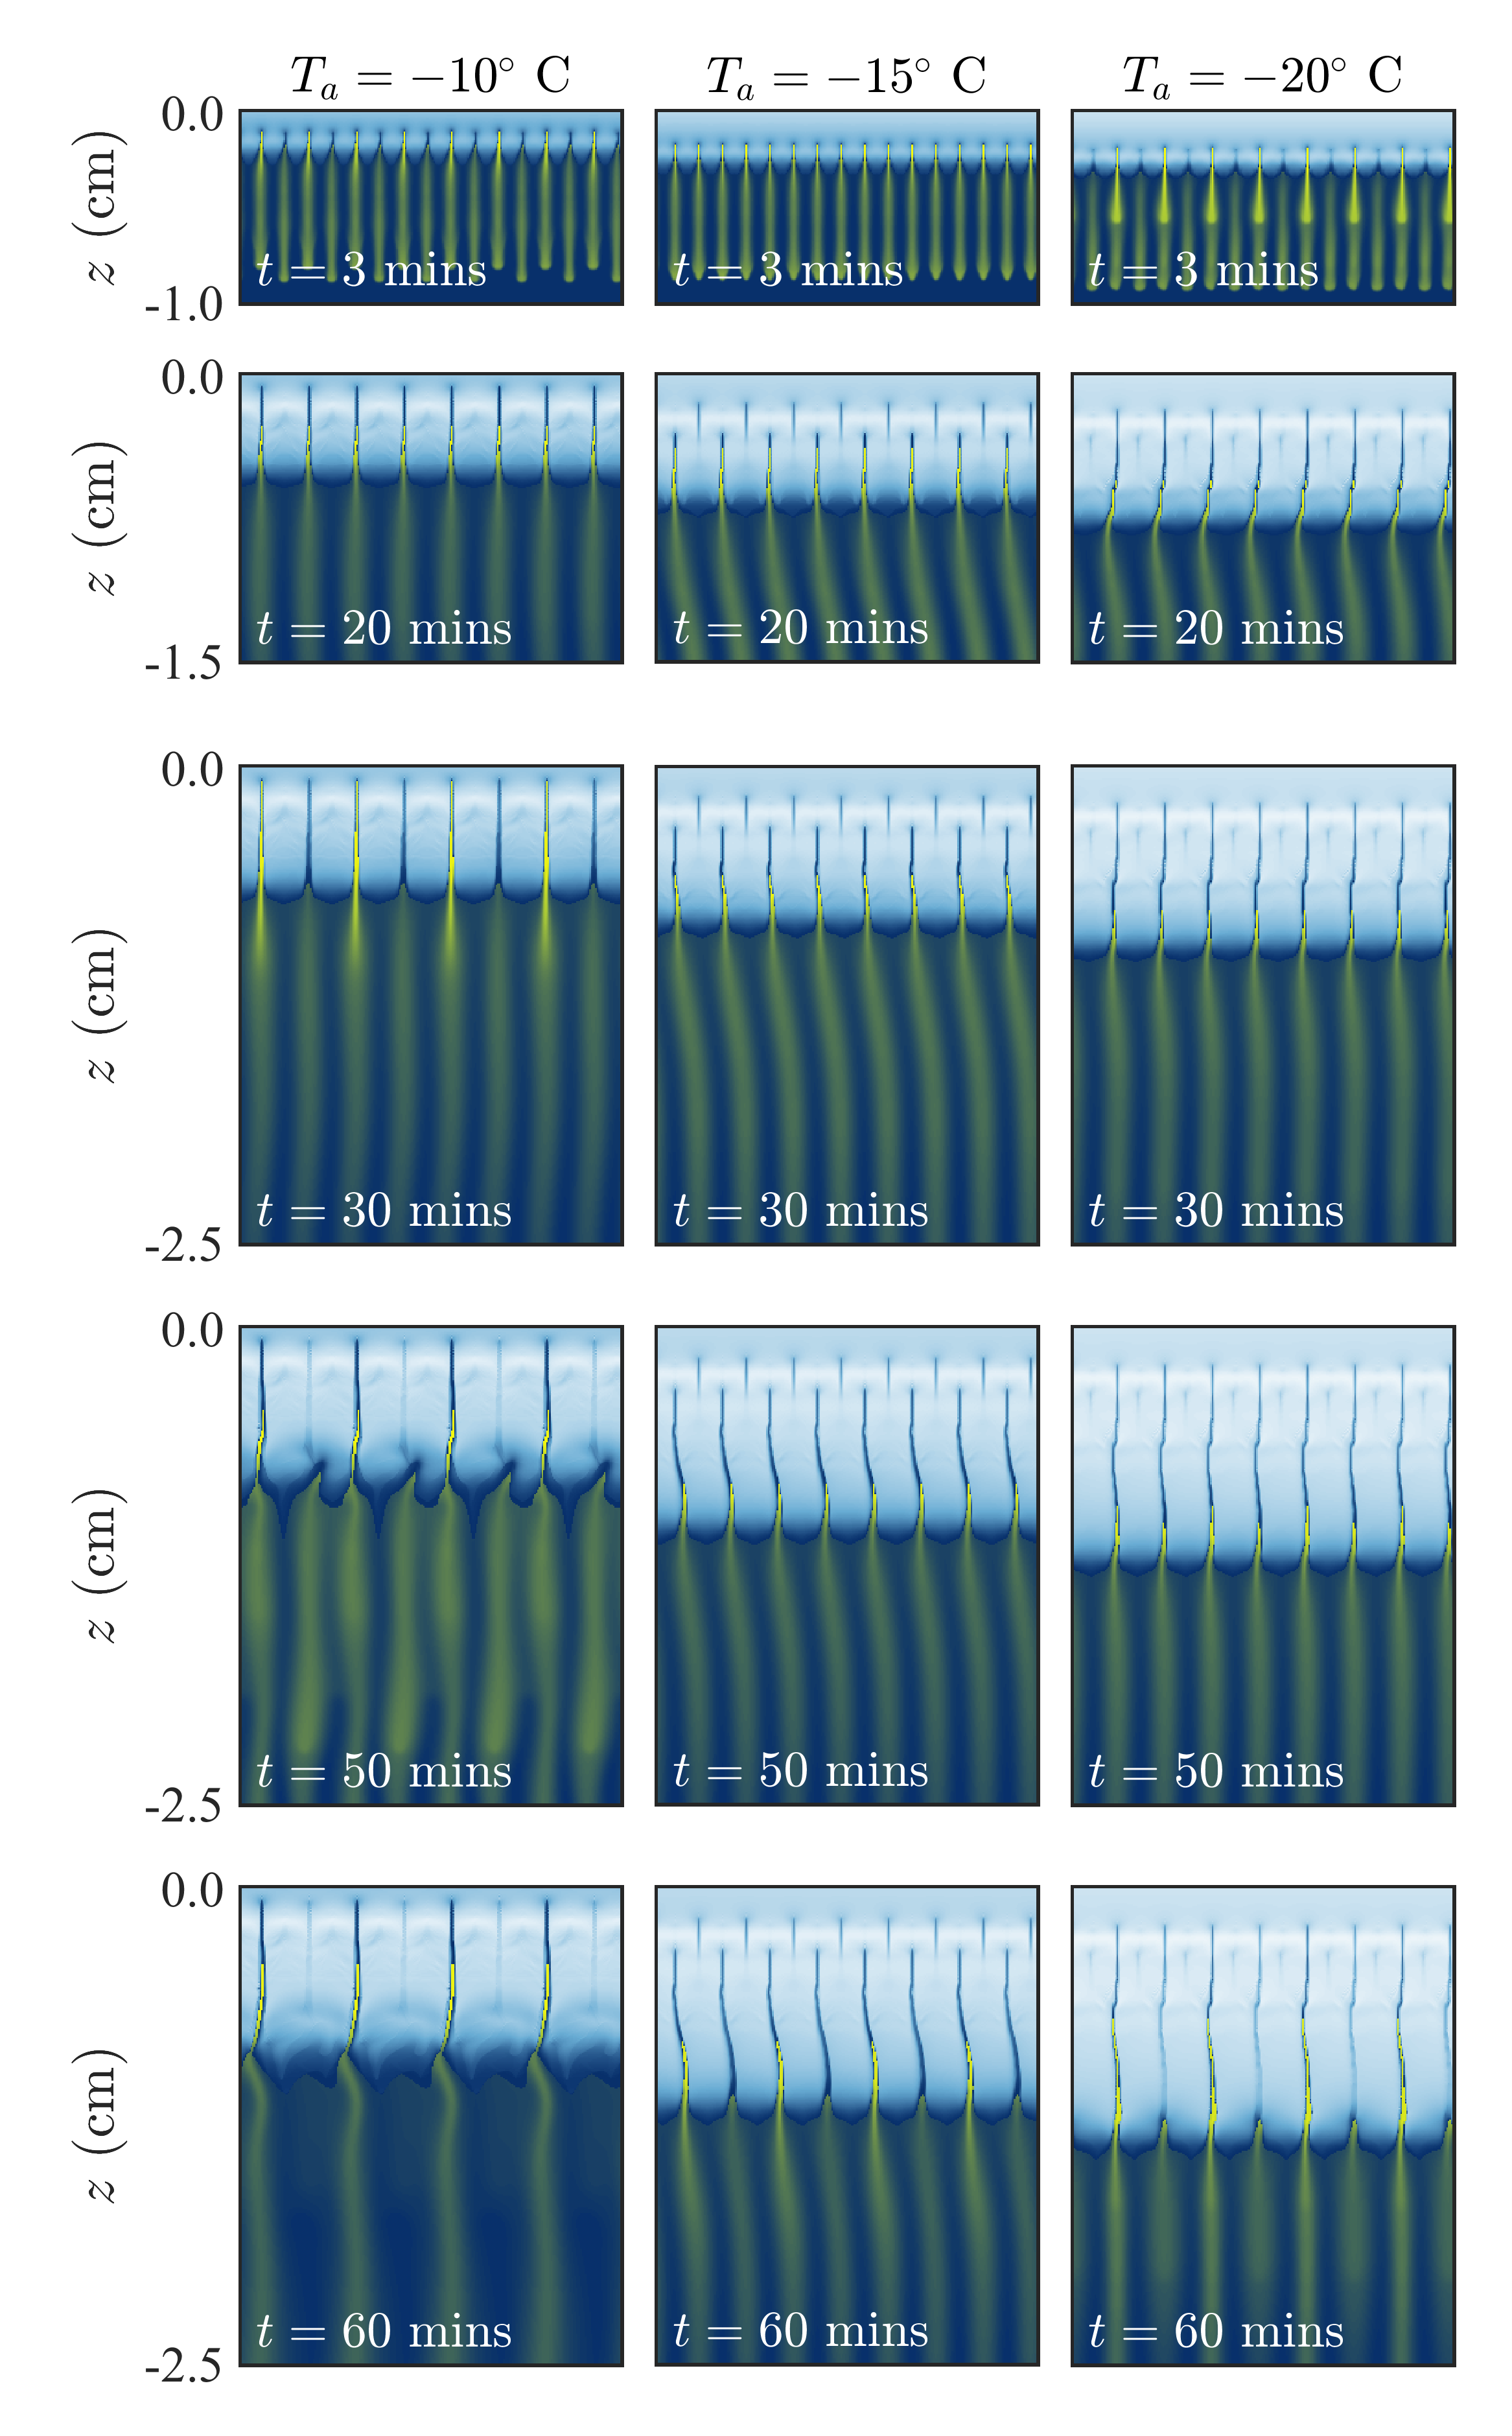
\includegraphics[width=30cm, trim={0.0cm, 0.5cm, 0.5cm, 0.5cm}, clip]{figures/timeSeries-t.png} };
%\node[anchor=south, inner sep=0pt, outer sep=0pt] (timeseries) at ([xshift=2cm,yshift=-1.2cm]timeseries.south) 
%{Go to https://goo.gl/4n9STV or scan QR code for movie};
\node[anchor=north west, inner sep=0pt, outer sep=0pt] (timeseries) at (0,0) {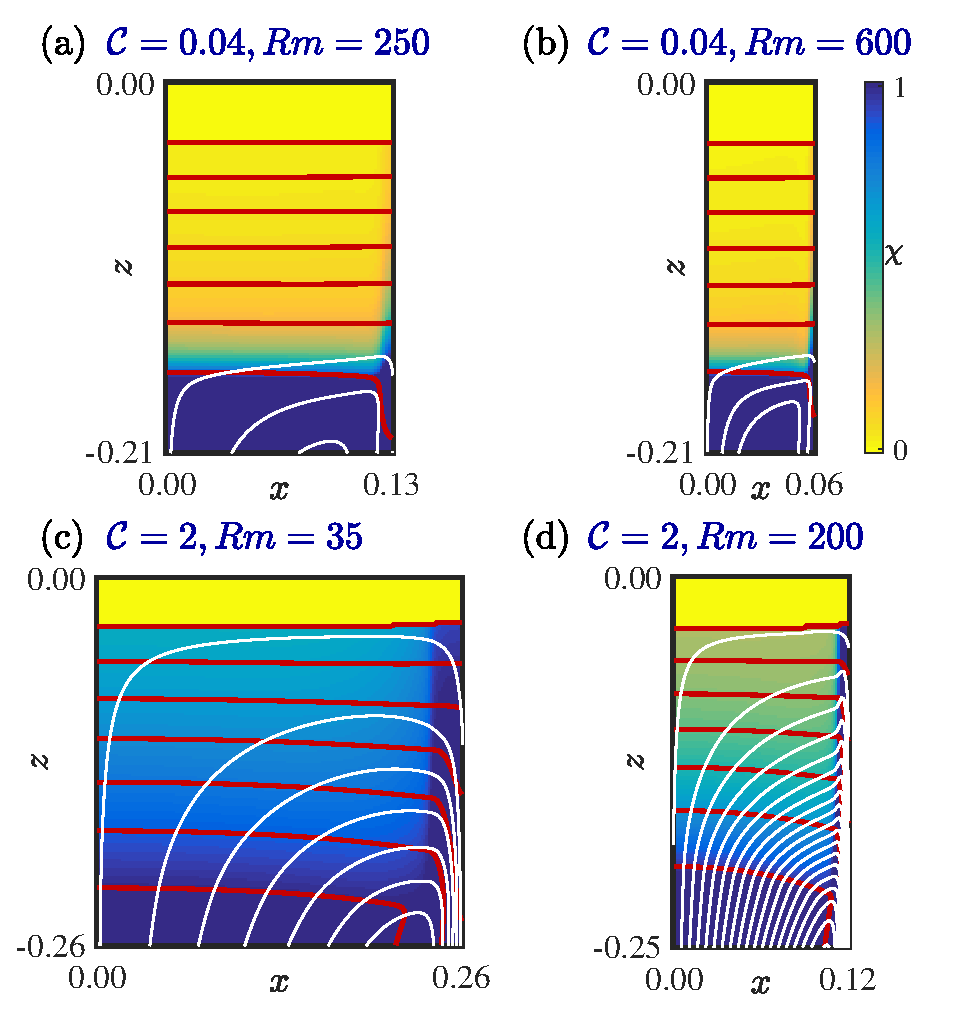
\includegraphics[width=0.95\linewidth, trim={0.0cm, 0.0cm, 0.2cm, 0.0cm}, clip]{figures/CRRaExampleSolutions.pdf} };
\end{tikzpicture}
\end{tikzfigure}
\end{minipage} 



 

\begin{tikzfigure}
\begin{tikzpicture}
\node[anchor=north west, inner sep=0pt, outer sep=0pt] (BCs) at (0,0) {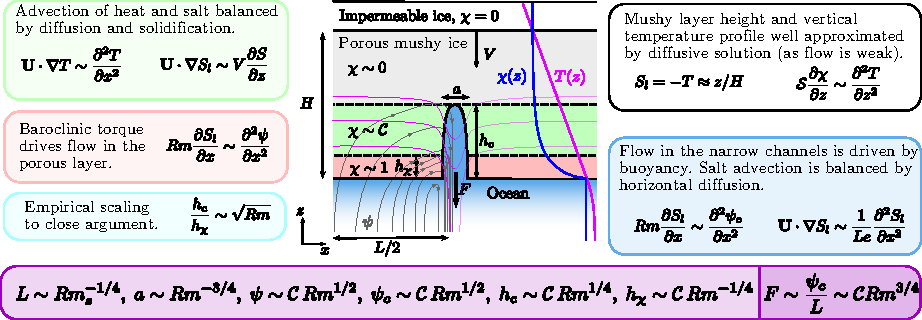
\includegraphics[width=\linewidth, trim={0.0cm, 0, 0, 0}, clip]{figures/scalingArgumentAnnotated.pdf} };

%\node[anchor=south west, inner sep=0pt, outer sep=0pt] (aLabel) at ([xshift=-0.5cm, yshift=-0.8cm]BCs.north west) {(a)};

%\node[anchor=south west, inner sep=0pt, outer sep=0pt] (bLabel) at ([xshift=0.5cm, yshift=-0.8cm]BCs.north) {(b)};
\end{tikzpicture}
\end{tikzfigure}

\vspace{-2em}

 
%% Validation of scaling laws
\begin{minipage}[t]{0.42\linewidth}
\begin{tikzfigure}
\label{fig:fluxScaling}
\begin{tikzpicture}

\node[anchor=north west] (fig1) at (0,0) {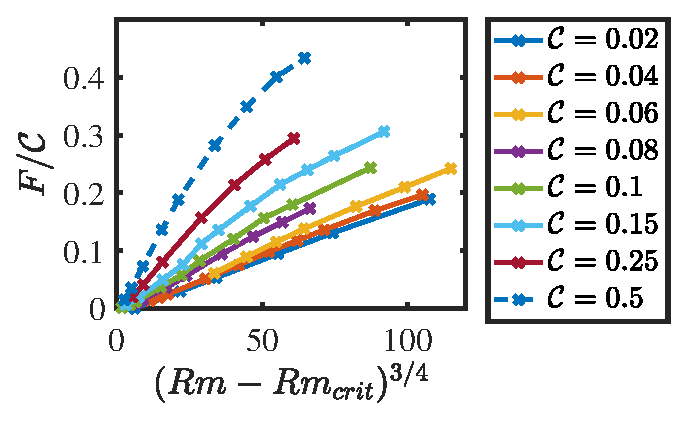
\includegraphics[height=11cm, trim={0.0cm, 0.0cm, 0.0cm, 0.0cm}, clip]{figures/fluxScalingPoster.eps} };
 
\end{tikzpicture}
\end{tikzfigure}
%Fig. x: Numerically calculated porosity (color scale and black contours), liquid salinity (magenta), and streamlines (gray, clockwise) for ice grown from 30 g/kg salt water with $\RmS=400$. 
\figureTitle{Fig. 7:}\figureCaption{Numerically calculated \highlightText{salt flux increases nearly linearly with $(\Rm - \Rm_{crit})^{3/4}$} when $\mathcal{C} \ll 1$, where $\Rm_{crit}$ is the critical Rayleigh number for convection.}
\end{minipage} \hfill
\begin{minipage}[t]{0.55\linewidth}
\begin{tikzfigure}
\label{fig:WWH}
\begin{tikzpicture}

\node[anchor=north west] (fig1) at (0,0) {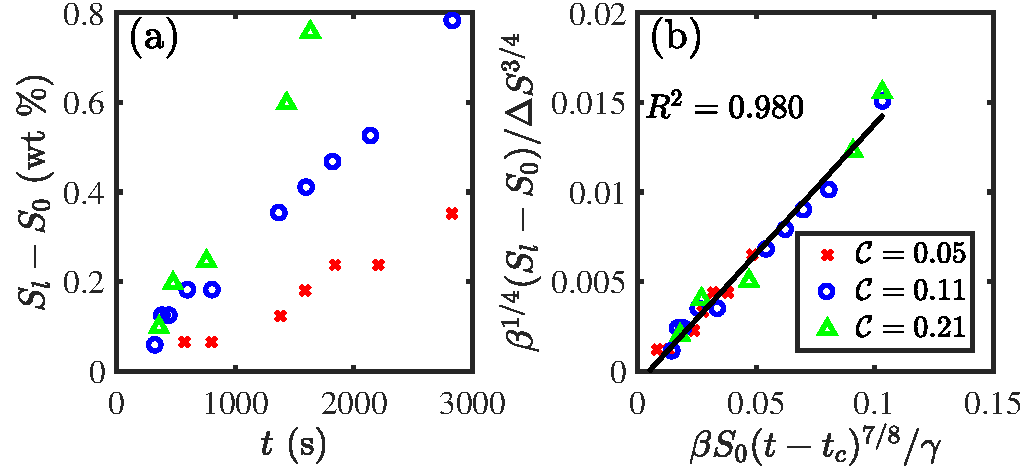
\includegraphics[height=11cm, trim={0.0cm, 0.0cm, 0.0cm, 0.0cm}, clip]{{figures/WWHPosterCollapse-LiquidusSlope-0.1}.pdf} };    
 
\end{tikzpicture}
\end{tikzfigure}


\figureTitle{Fig. 8:}\figureCaption{(a) Change in salinity of the underlying liquid  during transient growth measured by \cite{wettlaufer-et-al-97}. (b) Collapse of the data predicted by $F\sim \mathcal{C} Rm^{3/4}$, where $t_c$ is the time when convection starts and $\gamma = l \; \kappa_l^{-3/8} \left(g K_0/\nu \right)^{-3/4}$.}
\end{minipage}

\end{tcolorbox}

\vspace{-0.9em}} % end big main block

\begin{subcolumns}  
\subcolumn{0.77} 



\block{Governing Equations for Flow in Porous Mushy Sea Ice}
{
%Continuous equations for conservation of momentum, mass, energy, and salt are found by averaging over lengths greater than the pore scale of sea ice \cite{Worster1991} and nondimensionalised. For flow in a narrow Hele-Shaw cell, the momentum equation is well approximated by Darcy's law everywhere. \\
Solve for flow and solidification in reactive porous media \cite{Worster1991} with Darcy's law applied in a narrow Hele-Shaw cell with variable ice porosity. \\
Scales: length $\sim l$, time $\sim l^2/\kappa_l$, velocity $\sim \kappa_l/l$, temperature $\Delta T \sim T_e-T_0$, salinity $\Delta S \sim S_e-S_0$, permeability $\sim K_0$, pressure $\sim \eta \kappa_l / K_0$.



\begin{minipage}[t]{0.55\linewidth}
 \vspace{-0.1em}
\begin{minipage}[t]{6cm}
\eqnLabel{Momentum}
\end{minipage}
\begin{minipage}[t]{0.4\linewidth}
\vspace{-1.5em}
\begin{align} 
    \mathbf{U} = Rm \Pi \left(-\nabla p - S_l \right), \nonumber
  \end{align}
\end{minipage} \hfill \\
\begin{minipage}[t]{6cm}
\vspace{0.25em}
\eqnLabel{Energy}
\end{minipage}
\begin{minipage}[t]{0.4\linewidth}
\vspace{-0.5em}
\begin{align} 
    \frac{D H}{Dt} + \mathbf{U} \cdot \nabla T = \nabla \cdot \left[\chi + (1-\chi) k \right] \nabla T , \nonumber \label{eq:energy-cons} 
  \end{align}
\end{minipage} \hfill \\
\begin{minipage}[t]{6cm}
\vspace{1em}
\eqnLabel{Mass, salt}
\end{minipage}
%\hfill
\begin{minipage}[t]{0.48\linewidth}
\vspace{-0.0em}
\begin{align} 
    \nabla \cdot \mathbf{U} = 0, \hspace{10ex} \frac{D S}{Dt} + \mathbf{U} \cdot \nabla S = \Le^{-1} \nabla \cdot \chi \nabla S. \nonumber
     \end{align}
\end{minipage} \hfill \\
%\vspace{0.3em}
%\textcolor{dividingLines}{\hrule}
%\vspace{0.3em}
\begin{minipage}[t]{6cm}
\vspace{1.2em}
\eqnLabel{Parameters}
\end{minipage}
%\hspace{-5em} 
\begin{minipage}[t]{0.78\linewidth}
\vspace{0.2em}
\begin{align} 
   \textcolor{dukeblue}{ Rm = \frac{ \, \rho_0 \, g \, \beta \, \Delta S \, K_0 \,l}{\kappa_l \, \eta}}, \;\; Le = \frac{\kappa_l}{D_l}, \; \;St = \frac{L}{c_{p,l} \Delta T}, \; \; c_p = \frac{c_{p,s}}{c_{p,l}}, \; \; k = \frac{k_{s}}{k_{l}}. \nonumber
\end{align}
\end{minipage}

\iffalse
\begin{minipage}{\linewidth}
\begin{minipage}[t]{0.2\linewidth}
Length: $\sim l$.  \\
Time: $ \sim l^2/ \kappa_l$.
\end{minipage}
\begin{minipage}[t]{0.35\linewidth}
Permeability: $\sim K_0$.  \\
Pressure: $ \sim (\rho_0 K_0 / \eta^2)$.
\end{minipage}
\begin{minipage}[t]{0.45\linewidth}
%Temperature, salinity: $(T,S)_\text{eutectic} - (T,S)_0$. \\
Temperature: $\Delta T = \sim T_e - T_0$. \\
Salinity: $\Delta S \sim S_e - S_0$. 
\end{minipage}
\end{minipage}
\begin{minipage}{0.9\linewidth} % 0.9 here forces minipage to the left
\begin{align} 
   & \mathbf{U} = Rm \Pi \left(-\nabla p - S_l \right), \quad \frac{D H}{Dt} + \mathbf{U} \cdot \nabla T = \nabla \cdot \left[\chi + (1-\chi) k \right] \nabla T , \nonumber  \\
   & \nabla \cdot \mathbf{U} = 0, \hspace{15ex} \frac{D S}{Dt} + \mathbf{U} \cdot \nabla S = \Le^{-1} \nabla \cdot \chi \nabla S. \nonumber \\
   & Rm = \frac{\beta \, \rho_0 \, g \, \Delta S \, K_0 \,l}{\kappa_l \, \eta}, \;\; Le = \frac{\kappa_l}{D_l}, \; \;St = \frac{L}{c_{p,l} \Delta T}, \; \; c_p = \frac{c_{p,s}}{c_{p,l}}, \; \; k = \frac{k_{s}}{k_{l}}. \nonumber
\end{align}
\end{minipage}
\fi
\end{minipage} \hfill
\begin{minipage}[t]{0.4\linewidth}
\vspace{-1.2\baselineskip}
\begin{align*}
&\varColor{\mathbf{U}}\; \varLabel{(Darcy velocity)}, \quad \varColor{\chi} \; \varLabel{(porosity)}, \quad \varColor{p} \; \varLabel{(pressure)}, \quad \varColor{T} \; \varLabel{(temperature)},\\
&\varColor{S_l} \; \varLabel{(liquid salinity)}, \quad \varColor{S = \chi S_l} \; \varLabel{(bulk salinity)},  \\
&\eqnColor{H = St \chi + \left[\chi + (1-\chi) c_p \right] T} \; \varLabel{(enthalpy)}, \\
%&\eqnColor{H = \rho_0 \left\{ L \chi + \left[\chi c_{p,l} + (1-\chi) c_{p,s}\right] T \right\}} \; \varLabel{(enthalpy)}, \\
&\eqnColor{\Pi(\chi)^{-1} = \Pi_\text{Hele-Shaw}^{-1} + \chi^{-3}} \; \varLabel{(permeability)}, \\
&\paramColor{\eta} \; \varLabel{(viscosity)}; \paramColor{D_l} \; \varLabel{(salt diffusivity)};\paramColor{\beta} \; \varLabel{(haline expansion)}; \\
&\paramColor{c_{p,l}}, \paramColor{c_{p,s}} \; \varLabel{(liquid/solid specific heat)}; \paramColor{k_l}, \paramColor{k_s} \; \varLabel{(liquid/solid heat conductivity)}; \\
&\paramColor{d} \; \varLabel{(Hele-Shaw cell thickness)}; \paramColor{K_0} \; \varLabel{(reference permeability)}; \\
&\paramColor{l} \; \varLabel{(box height)}; \; \paramColor{\kappa_l} \; \varLabel{(liquid heat diffusivity)}; \; \paramColor{\rho_0} \; \varLabel{(reference density)}.
\end{align*}
\vspace{-1.9em}
\end{minipage}

%\begin{minipage}[t][][b]{0.48\linewidth}
%\begin{align*}
%&\mathbf{U}\; \text{(Darcy velocity)}, \quad \chi \; \text{(porosity)}, \quad \Pi \; \text{(permeability)}, \quad p \; \text{(pressure)}, \\
%&H = \chi S_t + T \; \text{(enthalpy)},\quad T \; \text{(temperature)}, \quad S \; \text{(salt concentration)}, \\
%&Ra - \text{Rayleigh number, determining the importance of buoyancy}, \\
%&Da - \text{Darcy number, determining the importance of viscosity}, \\
%&Le - \text{Lewis number, ratio of heat diffusion to salt diffusion}, \\
%&S_t - \text{Stefan number, quantifies energy release during freezing}.
%\end{align*}
%\end{minipage}

% \iffalse
% Continuous equations for conservation of momentum~\eqref{eq:mom-cons}, mass~\eqref{eq:mass-cons}, salt~\eqref{eq:energy-cons} and energy~\eqref{eq:salt-cons} are found by averaging over lengths greater than the pore scale of sea ice \cite{Worster1991,LeBars2006}. \\
% \begin{minipage}[t]{0.49\linewidth}
% \begin{align}
%      \rho_0  \frac{\partial \mathbf{U}}{\partial \tau} + \rho_0 \mathbf{U} \cdot \nabla \left( \frac{\mathbf{U}}{\chi} \right) &= - \chi \nabla p + \eta \nabla^2 \mathbf{U} + \chi \rho_l \mathbf{g} - \frac{\eta \chi}{K(\chi)} \mathbf{U},  \\
%   \nabla \cdot \mathbf{U} &= 0, \label{eq:mass-cons}  \\
%     \frac{\partial S}{\partial t} + \mathbf{U} \cdot \nabla S_l &= \nabla \cdot \chi D_l \nabla S_l, \label{eq:salt-cons} \\
%     \frac{\partial H}{\partial t} + \rho_0 \, c_{p,l} \, \mathbf{U} \cdot \nabla  T &= \nabla \cdot \left[ k_l \chi + (1-\chi) k_s \right] \nabla T . \label{eq:energy-cons}
% \end{align} 
% \end{minipage}
% \hfill
% \begin{minipage}[t][][b]{0.48\linewidth}
% \vspace{-1.75\baselineskip}
% \begin{align*}
% &\varColor{\mathbf{U}}\; \text{(Darcy velocity)}, \quad \varColor{\chi} \; \text{(porosity)}, \quad \varColor{p} \; \text{(pressure)}, \quad \varColor{T} \; \text{(temperature)},\\
% &\varColor{S_l} \; \text{(liquid salinity)}, \quad \varColor{S = \chi S_l} \; \text{(bulk salinity)},  \\
% &\eqnColor{H = \rho_0 \left\{ L \chi + \left[\chi c_{p,l} + (1-\chi) c_{p,s}\right] T \right\}} \; \text{(enthalpy)}, \\
% &\eqnColor{\rho_l = \rho_0 \left[1 - \alpha T + \beta S_l \right]} \; \text{(liquid density)}, \\
% &\eqnColor{K(\chi)^{-1} = \left(d^2/12\right)^{-1} + \left[K_0 \chi^3 / (1-\chi)^2 \right]^{-1}} \; \text{(permeability)}, \\
% &\paramColor{\eta} \; \text{(viscosity)}; \paramColor{D_l} \; \text{(salt diffusivity)}; \paramColor{\alpha}, \paramColor{\beta} \; \text{(thermal/haline expansion)}; \\
% &\paramColor{c_{p,l}}, \paramColor{c_{p,s}} \; \text{(liquid/solid specific heat)}; \paramColor{k_l}, \paramColor{k_s} \; \text{(liquid/solid heat conductivity)}; \\
% &\paramColor{d} \; \text{(Hele-Shaw cell thickness)}; \paramColor{K_0} \; \text{(Reference permeability)}.
% \end{align*}
% \end{minipage}
% \fi

}
 

\subcolumn{0.23}
 
 \block{Future Work}
{
\begin{itemize}
\item Consider growth over longer time periods (days to weeks), with time varying atmospheric forcing.
\item Simulations with the liquid region governed by the Navier-Stokes equation, rather than flow in a Hele-Shaw cell.
\item Three dimensional simulations, utilising the Adaptive Mesh Refinement capabilities of our code.
%\item Investigation of salt fluxes from warming sea ice in the spring/summer.
%\item Investigate salt fluxes over longer time periods, and with time dependent atmospheric forcing.
%\item Simulations with a liquid region governed by eq (1), rather than flow in a Hele-Shaw cell.
%\item Simulations in three dimensions, including Adaptive Mesh Refinement.
\end{itemize}
}

 
\end{subcolumns}

\end{columns}

\end{document}
